\documentclass[12pt,a4paper]{report}

\usepackage{times}
\usepackage[german]{babel}
\usepackage{graphics}
\graphicspath{ {../img/} {../graph/img/} }
\usepackage{color}
\usepackage{ntheorem}
\theoremstyle{break}
\theorembodyfont{\normalfont}
\theoremprework{\bigskip\hrule\leavevmode}
\theorempostwork{\nopagebreak\hrule\leavevmode}
\newtheorem{exercise}{Aufgabe}[section]
\theoremstyle{plain}
\theoremprework{\bigskip\hrule\leavevmode}
\theorempostwork{\nopagebreak\hrule\leavevmode}
\newtheorem{proof}{Satz}[section]
\renewcommand{\labelenumii}{\arabic{enumi}.\arabic{enumii}.}
\newcommand{\algostep}[2]{\parbox{4cm}{\scalebox{0.5}{\includegraphics{#1}}}
  \hfill
  \parbox{7cm}{#2}
}
\title{Minimale Spannb\"{a}ume}
\author{Gabriel Katz\\ Matthias Neeracher}

\begin{document}
\maketitle
\tableofcontents
\chapter{Einleitung}

\section{Wie kann hier gearbeitet werden?}

Dieser Text wird Sie mit einem wichtigen algorithmischen Problem
bekannt machen: dem Finden eines minimalen Spannbaums. Im n\"{a}chsten
Unterkapitel finden Sie eine Einf\"{u}hrung in das Thema, doch bevor
Sie loslegen, soll Ihnen hier noch kurz der Aufbau des Textes und die
Arbeitsweise damit erl\"{a}utert werden.

Die folgenden Kapitel sind zur selbstst\"{a}ndigen Bearbeitung
gedacht. Sie werden zuerst kurz Ihre Kenntnisse von ungerichteten
Graphen nochmals auffrischen, lernen dann die Theorie von B\"{a}umen
und gerichteten Graphen kennen, und lernen dann zwei verschiedene
Algorithmen, um einen \emph{minimalen Spannbaum} zu finden.
 
Wenn Sie einige dieser Begriffe jetzt noch nicht verstehen, macht das
nichts. Mitbringen sollten Sie aber die folgenden Kenntnisse:

\begin{itemize}
\item Sie wissen, was ein Algorithmus ist.
\item Sie kennen die Grundbegriffe ungerichteter Graphen (wir werden
  diese allerdings in Kapitel~\ref{graphs} kurz repetieren).
\end{itemize}

Zur behandelten Theorie finden Sie immer auch Aufgaben, anhand derer
Sie das Gelernte pr\"{u}fen k\"{o}nnen. Die L\"{o}sungen dieser Aufgaben stehen
jeweils im zweitletzten Unterkapitel f\"{u}r jedes Thema. Das letzte
Unterkapitel ist dann der Kapiteltest, den Sie bearbeiten und mit
Ihrer Lehrperson besprechen sollten.

\newpage
\section{Worum geht es hier?}

In den fr\"uhen 20er Jahren besch\"aftigte sich der 
Mathematiker Otakar Bor\r{u}vka mit dem Problem, ein Gebiet (40
St\"{a}dte in S\"{u}d-M\"{a}hren) m\"{o}glichst effizient mit 
Elektrizit\"{a}t zu erschliessen.

\begin{figure}[h!]
\resizebox{!}{4cm}{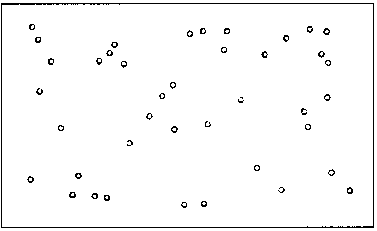
\includegraphics{BoruvkaPoints.pdf}}
\resizebox{!}{4cm}{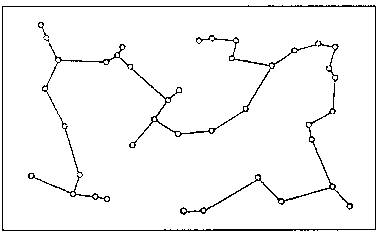
\includegraphics{BoruvkaTree.pdf}}
\caption{Elektrische Erschliessung von S\"{u}d-M\"{a}hren.\protect\footnotemark}
\end{figure}

\footnotetext{ 
Otakar  Bor\r{u}vka, \emph{O jist\'{e}m probl\'{e}mu minim\'{a}ln\'{i}m} (\"{U}ber ein
  gewisses Minimalisierungsproblem). \\
Zitiert aus: J. Ne\v{s}et\v{r}il,
  E. Milkov\'{a}, H. Ne\v{s}et\v{r}ilov\'{a}, \emph{Otakar Bor\r{u}vka
    on minimum spanning tree problem: translation of both the 1926
    papers, comments, history.}, Discrete Mathematics 233 (201)}
Sein Ansatz war, das Problem als Graphen abzubilden, in dem die
anzuschliessenden St\"{a}dte als Knoten, und die Distanzen zwischen ihnen
als Kanten repr\"{a}sentiert wurden. Das Elektrifizierungsproblem
besteht somit darin, alle Knoten so zu verbinden, dass die
Gesamtl\"{a}nge der Kanten so kurz wie m\"{o}glich bleibt. Eine solche
Verbindung wird \textbf{minimal aufspannender Baum} oder kurz
\textbf{minimaler Spannbaum} genannt.

Bor\r{u}vka's L\"{o}sung, die er 1926 publizierte, gilt als der erste
Algorithmus zur Konstruktion eines minimalen Spannbaums, und als einer
der ersten Optimierungs-Algorithmen. Weil sowohl
die Problemstellung als auch die verwendeten Algorithmen interessant
und einigermassen leicht verst\"{a}ndlich sind, werden wir uns jetzt diesem Problem widmen.

\chapter{Graphen}
\label{graphs}

\section{Rekapitulation: Was ist ein Graph?}

Ein \textbf{Graph} $G(V,E)$ besteht aus einer Menge von
\textbf{Knoten} $V$ und einer Menge von Kante $E$. Eine \textbf{Kante}
besteht aus einem Paar von Knoten, den \textbf{Endknoten} der
Kante. Wenn diese Paare geordnet sind, ist der Graph
\textbf{gerichtet}; die Kanten verbinden die Knoten nur in eine
Richtung. 

In diesem Text befassen wir uns aber nur mit
\textbf{ungerichteten} Graphen, in welchen die Knotenpaare ungeordnet
und somit die Knoten symmetrisch verbunden sind.  Des weiteren
beschr\"{a}nken wir uns auf \textbf{schlichte} Graphen, in denen keine
Kanten einen Knoten mit sich selbst verbinden, und zwischen zwei
Knoten nicht mehr als eine Kante existiert.

\begin{exercise}
Welche dieser vier Graphen sind gerichtet, welche ungerichtet? Welche
sind schlicht?

\scalebox{0.4}{\includegraphics{UngerichtetUnschlicht.pdf}}
\scalebox{0.4}{\includegraphics{Gerichtet.pdf}}
\scalebox{0.4}{\includegraphics{Ungerichtet.pdf}}
\scalebox{0.4}{\includegraphics{GerichtetUnschlicht.pdf}}
\end{exercise}

\section{Beschreibung von Graphen}
\label{Beschreibung}
\noindent Ein Graph $G(V,E)$ kann auf verschiedene Arten beschrieben werden:

\begin{description}
\item[Grafisch] indem die Knoten und Kanten aufgezeichnet werden:

\scalebox{0.5}{\includegraphics{Ungerichtet.pdf}}

gerade bei kleineren Graphen ist diese Darstellung f\"{u}r Menschen am
Einfachsten zu verstehen, aber sie ist z.B. f\"{u}r
Computerverarbeitung nicht besonders gut geeignet.
\item[Mengentheoretisch] indem die Knoten- und die Kantenmenge
  beschrieben werden:

\begin{displaymath}
V = \{\mathsf{A,B,C,D,E}\}\hspace{2cm}E = \{\mathsf{(A,B), (B,C),
  (C,D), (C,E), (B,E)}\}
\end{displaymath}

\item[\textnormal{als} Adjazenzmatrix] indem die Kanten als $n\times{n}$ Matrix $A(G)$
  dargestellt werden, wo der Eintrag $a_{ij}$ gleich $1$ ist, wenn eine Kante
  von Knoten $i$ nach Knoten $j$ existiert, und sonst gleich $0$.

\begin{displaymath}
A(G) = \left( 
\begin{array}{ccccc}
0 & 1 & 0 & 0 & 0 \\
1 & 0 & 1 & 0 & 1 \\
0 & 1 & 0 & 1 & 1 \\
0 & 0 & 1 & 0 & 0 \\
0 & 1 & 1 & 0 & 0 
\end{array}
\right)
\end{displaymath}

Wie zu beobachten ist, ist die Adjazenzmatrix bei einem ungerichteten
Graphen immer symmetrisch.
\end{description}

\begin{exercise}
\begin{itemize}
\item Zeichnen Sie einen ungerichteten Graphen $G(V,E)$ mit Knoten 
$V = \{\mathsf{A,B,C,D,E}\}$ und Kanten 
$E = \{\mathsf{(A, B), (A, D), (C, D), (A, E)}\}$.
\item Konstruieren sie die Adjazenzmatrix dieses Graphen.
\end{itemize}
\end{exercise}

\section{Zusammenh\"{a}ngende Graphen}

Wenn in einem Graphen $G(V,E)$ eine Folge von Knoten $v_0, v_1,
\ldots, v_n \in V$ existiert, die von Kanten $e_i = (v_i, v_i+1) \in
E$ verbunden werden, dann existiert ein \textbf{Weg} von $v_0$ nach
$v_n$. 

Falls ein Weg f\"{u}r \emph{jedes} Knotenpaar $v_0, v_n
\in V$ existiert, nennen wir den Graphen \textbf{zusammenh\"{a}ngend}.

Ein Weg $v_0\cdots{v_1}\cdots\ldots\cdots{v_0}$, der von einem Knoten
$v_0$ wieder auf diese selbst zur\"{u}ckf\"{u}hrt, heisst
\textbf{geschlossen}. Ein \textbf{zyklischer} Graph besteht aus einen
geschlossenen Weg, der alle Knoten und alle Kanten enth\"{a}lt.

\begin{exercise}
\textcolor{red}{Irgendwelche Ideen?}
\end{exercise}

\section{Untergraphen}

Ein Graph $U(W,F)$ ist ein \textbf{Untergraph} eines Graphen $G(V,E)$
wenn seine Knotenmenge $W$ eine Untermenge der Knotenmenge $V$ ist und
seine Kantenmenge $F$ eine Untermenge der Kantenmenge $E$.

\begin{exercise}
Welche der folgenden drei Graphen sind Untergraphen des Graphen in
Abschnitt~\ref{Beschreibung} ?

\scalebox{0.4}{\includegraphics{Sub1.pdf}}
\scalebox{0.4}{\includegraphics{Sub2.pdf}}
\scalebox{0.4}{\includegraphics{Sub3.pdf}}

\end{exercise}
\begin{exercise}
\textbf{FAKULTATIV} Wie viele Untergraphen $\mathcal{U}_n$ hat ein
\emph{vollst\"{a}ndiger} Graph 
\[ 
G(V = \{v_1, v_2, \ldots, v_n\}, E = \{(v_a, v_b) \mid v_a, v_b \in V,
v_a \neq v_b\}) ?
\] 
Finden Sie eine rekursive Definition $\mathcal{U}_n = f(\mathcal{U}_{n-1})$.
\end{exercise}

\newpage
\section{Gewichtete Graphen}
\label{gewichtet}

In vielen praktischen Anwendungen sind die Knoten und/oder Kanten
eines Graphen mit \textbf{Gewichten} versehen. Die Kantengewichte k\"{o}nnen
z.B. Distanz oder Flugkosten darstellen, die Knotengewichte
z.B. Hotelkosten.

\begin{exercise}
\label{travel}
Der folgende Graph zeigt Flug- und Hotelkosten, sowie Reisedistanzen
f\"{u}r eine Reise.

\scalebox{0.5}{\includegraphics{Travel.pdf}}

\begin{itemize}
\item Was ist die \emph{k\"{u}rzeste} Route zwischen Z\"{u}rich und
    Sydney?
\item Was ist die \emph{billigste} Route?
\end{itemize}
\end{exercise}

 In der weiteren Diskussion werden wir hier nur noch an \textbf{Kantengewichteten} Graphen interessiert sein.

\section{L\"{o}sungen}

\textcolor{red}{To Be Completed}

\section{Kapiteltest}

\textcolor{red}{To Be Completed}

\chapter{B\"{a}ume}

\section{Was ist ein Baum?}

Als \textbf{Baum} bezeichnet man einen Graphen, der
\emph{zusammenh\"{a}ngend} ist und \emph{keinen geschlossenen Weg}
enth\"{a}lt. Eine Menge von B\"{a}umen, die keine gemeinsamen Knoten
haben, bezeichnet man (anschaulicherweise) als \textbf{Wald}.

\textcolor{red}{Aufgaben: Baeume identifizieren}

\begin{proof}
Ein Baum mit $n$ Knoten hat exakt $n-1$ Kanten.

\bigskip\noindent\textsc{Beweis:} Ein Baum mit $1$~Knoten kann keine Kanten haben.
In einem Baum mit $n$~Knoten sucht man sich einen beliebigen Knoten
aus, folgt einer beliebigen Kante, und beim n\"{a}chsten Knoten sucht
man sich eine andere Kante aus.
Weil der Baum ja keinen geschlossenen
Weg enth\"{a}lt, landet man irgendwann in einem Knoten, der von nur
$1$~Kante erreicht wird. 
Wenn man diesen Knoten und seine Kante aus
dem Baum entfernt, erh\"{a}lt man einen Baum mit $n-1$~Knoten, und
durch Induktion l\"{a}sst sich sehen, dass der Satz gilt.
\end{proof}

\section{Spannb\"{a}ume}

F\"ur jeden zusammenh\"{a}ngenden Graphen $G(V,E)$ kann man einen oder mehrere
\textbf{Spannb\"{a}ume} konstruieren, die aus \emph{allen Knoten} $V$ des
Graphen und einer \emph{Untermenge der Kanten} $E$ bestehen.

\textcolor{red}{Aufgaben: Alle aufspannenden Baeume fast vollstaendiger 4-Graph}

\section{Minimale Spannb\"{a}ume}

Wenn wir jetzt wieder an das in Kapitel~\ref{gewichtet}
eingef\"{u}hrten Konzept des \emph{kantengewichteten Graphen}
zur\"{u}ckdenken, k\"{o}nnen wir dieses auch auf B\"{a}ume
anwenden. Das \textbf{Gewicht} eines Baumes l\"{a}sst sich dann als
Summe der Kantengewichte des Baumes definieren.

\textcolor{red}{Aufgabe: Gewicht}

Somit k\"{o}nnen wir nun den zentralen Begriff dieses Textes
definieren: Ein Spannbaum $B$ eines Graphen $G$ ist ein
\textbf{minimaler Spannbaum} von $G$ wenn kein Spannbaum von $G$
existiert, dessen Gewicht kleiner als das Gewicht von $B$ ist.

Ein Graph kann ohne weiteres mehrere minimale Spannb\"{a}ume haben:
Wenn z.B. alle Kantengewichte identisch sind, sind \emph{alle}
Spannb\"{a}ume minimal!

\textcolor{red}{Aufgaben}

\section{L\"{o}sungen}
\textcolor{red}{To Be Completed}
\section{Kapiteltest}
\textcolor{red}{To Be Completed}

\chapter{Algorithmen}

Wie findet man denn nun einen minimalen Spannbaum in einem
nicht-trivialen Graphen? In diesem Kapitel werden wir zwei
verschiedene Algorithmen kennenlernen, die dies bewerkstelligen.

\section{Gierige Algorithmen}

Ein Algorithmus wird \textbf{gierig} (bzw. das Englische Aequivalent
\textbf{greedy}) genannt, wenn er in jedem Schritt einen \emph{lokal
  optimalen} Folgezustand w\"{a}hlt. In Reiseproblem, das in
Aufgabe~\ref{travel} besprochen wurde, w\"{u}rde ein gieriger
Algorithmus z.B. in jedem Schritt den k\"{u}rzesten oder den
billigsten Flug aus der gegenw\"{a}rtigen Stadt in eine noch nicht
besuchte Stadt w\"{a}hlen.

Gierige Algorithmen sind oft einfach zu verstehen und schnell, aber
sie l\"{o}sen viele Probleme nicht optimal: In unserem Beispiel
w\"{u}rde der Algorithmus zwar den billigsten Weg finden, aber im
allgemeinen Fall ist das nicht garantiert, und der Algorithmus
w\"{u}rde hier die falsche L\"{o}sung f\"{u}r den k\"{u}rzesten Weg
finden.

Gl\"{u}cklicherweise ist das Finden eines minimalen Spannbaums eines
der Probleme, bei denen gierige Algorithmen ein optimales Resultat
garantieren k\"{o}nnen:

\begin{proof}\label{minimalkante}
  Es sei $G(V,E)$ ein kantenbewerteter
  zusammenh\"{a}ngender Graph. $U$ sei eine Teilmenge der Knoten $V$ und
  $e_{min}$ die Kante mit dem kleinsten Gewicht in der Kantenmenge
  $\{e=(u,v) \mid e\in E, u\in U, v\in (V\!\setminus\!U) \}$. Dann existiert ein
  minimaler Spannbaum von $G$, der $e_{min}$ enth\"{a}lt.

 \bigskip\noindent\textsc{Beweis:} Nehmen wir das Gegenteil an: $e_{min}$
liegt in \emph{keinem} minimalen Spannbaum von $G$. Wenn wir dann $B$,
einen beliebigen minimalen Spannbaum von $G$, nehmen und $e_{min}$ in $B$
einf\"{u}gen, erh\"{a}lt man einen geschlossenen Weg $W$ in $B$, der
$e_{min}$ enth\"{a}lt. Da $W$ Knoten sowohl aus $U$ als auch aus
$V\!\setminus\!U$ enth\"{a}lt, muss $W$ eine andere Kante $(u', v')$
enthalten, in der $u' \in U, v'\in (V\!\setminus\!U)$ sind. Wenn man
dann $(u',v')$ aus $B$ entfernt, bleibt der entstehende Baum $B'$ ein Spannbaum, und da nach
Definition das Gewicht von $e_{min}$ nicht gr\"{o}sser sein kann als
das von $(u',v')$, kann auch das Gewicht von $B'$ nicht
gr\"{o}sser sein als das von $B$: $B'$ muss ebenfalls ein minimaler
Spannbaum sein, und da $B'$ $e_{min}$ enth\"{a}lt, ist die
Gegenannahme widerlegt.

\textcolor{red}{Wollen wir diesen Beweis?}
\end{proof} 

\section{Der Algorithmus von Kruskal}

Der erste Algorithmus den wir behandeln wurde von dem
amerikanischen Mathematiker Joseph Kruskal entwickelt und erstmals
1956 publiziert. Der minimale Spannbaum f\"{u}r den Graphen $G(V,E)$
wird konstruiert, indem ein Wald $W(V, E')$ von minimalen B\"{a}umen
sukzessive verbunden wird, bis ein einziger minimaler Spannbaum
\"ubrigbleibt:

\begin{enumerate}
\item Der Anfangszustand des Waldes besteht aus einem Baum pro Knoten:
  $W \gets (V, \{\})$ (Beachten Sie, dass ein
  einzelner Knoten bereits einen Baum darstellt)
\item So lange es Kanten $K$, $K\subset (E\setminus{E'})$ gibt, die in $W$ noch nicht
  verwendet wurden, und die mit den verwendeten Kanten $E'$ keinen
  geschlossenen Weg bilden:
\begin{enumerate}
\item W\"{a}hlen Sie die Kante $e_i\in K$ mit dem kleinsten
  Kantengewicht aus.
\item F\"{u}gen Sie diese Kante zu $W$ hinzu: $E' \gets E'+\{e_i\}$.
\end{enumerate}
\end{enumerate}

\newpage
Hier soll ein einfaches Beispiel graphisch illustriert werden:

\algostep{Demo.pdf}{Der Anfangszustand, $E' = \{\}$}
\algostep{DemoKruskal1.pdf}{Schritt $1$: Eine der beiden Kanten mit Gewicht $5$
  (egal welche) wurde hinzugef\"ugt: $E' = \{(A,D)\}$}
\algostep{DemoKruskal2.pdf}{Schritt $2$: Die n\"{a}chstk\"{u}rzere
  Kante wurde hinzugef\"ugt: $E' = \{(A,D), (C,E)\}$}
\algostep{DemoKruskal3.pdf}{Schritt $4$: Nachdem zwei weitere Kanten
  hinzugef\"ugt wurden, wird jetzt klar, dass die Kante $(B,C)$ nie
  mehr hinzugef\"ugt werden wird, weil sie mit $(B,E)$ und $(C,E)$
  einen geschlossenen Weg bilden w\"{u}rde. $E' = \{(A,D), (B,E),
  (C,E), (D,F)\}$}

\newpage
\begin{exercise}
F\"{u}hren Sie den Algorithmus von Kruskal im vorstehenden Beispiel zu
Ende, bis der minimale Spannbaum konstruiert ist.
\end{exercise}

\begin{proof}\label{kruskproof}Der Algorithmus von Kruskal konstruiert
  einen minimalen Spannbaum.

\textcolor{red}{Beweis ist etwas komplex. Wollen wir ihn?}
\end{proof}

\section{Der Algorithmus von Prim}

Viele Optimierungsprobleme k\"{o}nnen auf viele verschiedene Arten
gel\"{o}st werden. Auch f\"{u}r das minimale Spannbaumproblem gibt es
viele Algorithmen, und wir wollen deshalb noch einen zweiten
Algorithmus vorstellen, um einen anderen Ansatz zu zeigen.

Dieser Algorithmus wurde bereits 1930 von dem Mathematiker
Vojt\v{e}ch Jarn\'ik entwickelt, geriet dann aber in Vergessenheit,
bis er 1957 von Robert C. Prim und 1959 von Edsger W. Dijkstra
unabh\"{a}ngig wiederentdeckt wurde (Aus diesem Grund ist der
Algorithmus auch unter anderen Namen, z.B. \emph{Prim-Dijkstra
  Algorithmus} oder \emph{Algorithmus von Jarnik, Prim, und Dijkstra}
bekannt).

Der Algorithmus von Prim konstruiert einen minimalen Spannbaum f\"{u}r
den zusammenh\"{a}ngenden Graphen $G(V,E)$ indem er einen bestehenden Baum $B(V_B,E_B)$
sukzessive durch Hinzuf\"{u}gen minimaler Kanten erweitert:

\begin{enumerate}
\item W\"{a}hlen Sie einen beliebigen Knoten $v_0\in V$ als
  Anfangszustand f\"{u}r $B$: $V_B \gets \{v_0\}$, $E_B \gets \{\})$.
\item Solange $V_B\neq V$:
\begin{enumerate}
\item W\"{a}hlen Sie unter den Kanten $\{e = (u,v)\mid u\in V_B, v\in
  (V\!\setminus\!V_B)\}$ die Kante $e_i= (u_i,v_i)$ mit dem kleinsten
Kantengewicht aus.
\item F\"{u}gen Sie die Kante und ihren Endpunkt zu $B$ hinzu: $V_B \gets
  V_B+\{v_i\}$, $E_B \gets E_B+\{e_{min}\}$.
\end{enumerate}
\end{enumerate}

\newpage
Auch hier werden wir das gleiche Beispiel illustrieren:

\algostep{DemoPrim1.pdf}{Der Anfangszustand, $V_B = \{A\}$ (beliebige
  Wahl), $E_B = \{\}$. M\"{o}gliche Erweiterungskanten sind $(A,B)$
  und $(A,D)$; letztere hat das kleinere Kantengewicht.}
\algostep{DemoPrim2.pdf}{Schritt $1$: $(A,D)$ bzw. $D$ wurden
  hinzugef\"{u}gt. $V_B = \{A,D\}, E_B=\{(A,D)\}$. Nun ist $(D,F)$ die
  beste Erweiterungskante.}
\algostep{DemoPrim3.pdf}{Schritt $2$: $(D,F)$ bzw. $F$ wurden 
 hinzugef\"{u}gt. $V_B = \{A,D,F\}, E_B=\{(A,D), (D,F)\}$. Nun kommt
 endlich $(A,B)$ als Erweiterungskante zum Zug.}

\begin{exercise}
F\"{u}hren Sie den Algorithmus von Prim im vorstehenden Beispiel zu
Ende, bis der minimale Spannbaum konstruiert ist.
\end{exercise}

\begin{proof}\label{primproof}Der Algorithmus von Prim konstruiert
  einen minimalen Spannbaum.

\textcolor{red}{Beweis ist etwas komplex. Wollen wir ihn?}
\end{proof}

\section{Schlussbetrachtung: Wer Gewinnt?}

Wenn mehrere verschiedene Algorithmen zur L\"{o}sung eines Problems
zur Wahl stehen, ist es eine naheliegende Frage, welcher davon denn
der effizienteste ist. Leider w\"{u}rde eine umfassende Erforschung dieser
Frage den Rahmen dieses Textes bei weitem sprengen, deshalb soll nur
kurz erw\"{a}hnt sein:

\begin{itemize}
\item Da alle Algorithmen hier optimale L\"{o}sungen finden,
  unterscheidet sich die Qualit\"{a}t der Resultate nicht.
\item Wenn man diese Algorithmen auf einem Computer programmiert,
  h\"{a}ngt deren Laufzeit- und Speichereffizienz enorm von den
  verwendeten Datenstrukturen ab, weil die Auswahl- und Testschritte
  (z.B. auf geschlossene Wege in Kruskal's Algorithmus, auf
  Mitgliedschaft von Knoten in Untergraphen in Prim's Algorithmus)
  entscheidend auf geeignete Datenrepr\"{a}sentation angewiesen sind.
\item In einer Studie von mehreren Implementierungen von Kruskal's und
  Prim's Algorithmus ist der Informatiker Donald
  E. Knuth\footnote{Donald E. Knuth, \emph{The Stanford GraphBase},
    Seiten 460--497} zum Schluss
  gelangt, dass sich die Effizienz der beiden Algorithmen nicht
  wesentlich voneinander unterscheidet.
\end{itemize}

\section{L\"{o}sungen}
\textcolor{red}{To Be Completed}
\section{Kapiteltest}
\textcolor{red}{To Be Completed}

\end{document}
